\documentclass[../notes.tex]{subfiles}

\pagestyle{main}
\renewcommand{\chaptermark}[1]{\markboth{\chaptername\ \thechapter\ (#1)}{}}
\renewcommand{\thechapter}{\Roman{chapter}}
\setcounter{chapter}{5}

\begin{document}




\chapter{Bonding and Physical Properties of Metal Complexes}
\section{Module 34: Magnetic Properties of Transition Metal Complexes}
\begin{itemize}
    \item \marginnote{2/22:}Electrons occupy the lowest energy triply degenerate orbitals in $d^1$, $d^2$, and $d^3$ configurations.
    \item However, in the $d^4$ configuration:
    \begin{itemize}
        \item Low spin: The fourth electron will pair up in the lower $t_{2g}$ energy level.
        \item High spin: The fourth electron will occupy a higher energy $e_g$ orbital.
    \end{itemize}
    \item The pairing energy $\Pi$ is made up of two parts (refer to Figure \ref{fig:coulombExchange} and the associated discussion):
    \begin{enumerate}
        \item Coulombic repulsion energy caused by having two eletrons in the same orbital. Destabilization energy contribution of $\Pi_c$ for each doubly occupied orbital. Has a positive sign because it increases the energy of the system.
        \item Exchange stabilization energy for each pair of electrons having the same spin and same energy. Stabilizing contribution of $\Pi_e$ for each pair having same spin and same energy. Has a negative sign because it reduces the energy of the system.
    \end{enumerate}
    \item Deciding whether the fourth electron will go into the higher energy $e_g$ orbital at an energy cost of $\Delta$, or be paired at an energy cost of $\Pi$.
    \begin{itemize}
        \item Strong field ligand has big $\Delta$ so $\Pi<\Delta$; this implies a low spin configuration.
        \item Weak field ligand has small $\Delta$ so $\Pi>\Delta$; this implies a high spin configuration.
    \end{itemize}
    \item We can experimentally discriminate between high- and low-spin compounds by measuring magnetic properties.
    \begin{itemize}
        \item The Gouy balance can determine the magnetic susceptibility of materials.
        \item A more modern way to measure magnetic properties uses a \underline{S}uperconducting \underline{Qu}antum \underline{I}nterference \underline{D}evice, or SQUID.
        \begin{itemize}
            \item This device is just about the most sensitive machine humanity can build (can detect the magnetic field of the heart/brain).
        \end{itemize}
    \end{itemize}
    \item Main types of magnetic behavior:
    \begin{itemize}
        \item Diamagnetism (from electron charge).
        \item Paramagnetism (spin and orbital motion of electrons on individual atoms).
        \item Ferromagnetism and antiferromagnetism (cooperative interaction between magnetic moments of individual atoms).
    \end{itemize}
    \item Paramagnetism is much stronger than diamagnetism and overpowers it.
    \begin{itemize}
        \item Ferromagnetism overpowers both.
    \end{itemize}
    \item Theoretical background for determining magnetic spins experimentally:
    \begin{itemize}
        \item When we place a sample in a magnetic field of magnitude $H$, the sample will interact with the magnetic field and magnetize. This magnetization causes the magnetic flux $B$ in the material to differ from the magnetic flux through the space the sample occupies (were the sample not there) by an amount determined by the magnetization parameter $M$, which is specific to each material. These three quantities are related via the equation
        \begin{equation*}
            B = H+4\pi M
        \end{equation*}
        \item If we divide the flux by the magnetic field, we obtain the magnetic susceptibility per unit volume $\kappa$ of the material:
        \begin{equation*}
            \frac{B}{H} = 1+4\pi\cdot\frac{M}{H} = 1+4\pi\kappa
        \end{equation*}
        \item This quantity can be normalized by the molecular weight and density of the substance to give the magnetic susceptibility per mole
        \begin{equation*}
            \chi_M = \kappa\cdot\frac{\text{molecular weight}}{\text{density}}
        \end{equation*}
        \item Dividing $\chi_M$ by Avogadro's number gives the magnetic susceptibility per molecule $\chi_M^\text{corr}$.
        \item \textbf{Curie's law} relates $\chi_M^\text{corr}$ to the magnetic moment $\mu$ by the formula
        \begin{equation*}
            \chi_M^\text{corr} = \frac{N\mu^2k}{3T}
        \end{equation*}
        where $N$ is Avogadro's number, $k=\SI[per-mode=symbol]{1.381e23}{\joule\per\kelvin}$ is the Boltzmann constant, and $T$ is the absolute temperature of the substance.
        \begin{itemize}
            \item Note that $\mu$ is measured in units of Bohr magnetons where $\SI{1}{B.M.}=\frac{eh}{4\pi m_ec}$. As per usual, we have $e=\SI{1.602e-19}{\coulomb}$ is the charge of an electron, $h=\SI{6.626e-34}{\joule\second}$ is Planck's constant, $m_e=\SI{9.11e-31}{\kilo\gram}$ is the mass of an electron, and $c=\SI[per-mode=symbol]{2.998e8}{\meter\per\second}$ is the speed of light.
            \item We can rearrange Curie's law to express the magnetic moment in terms of $\chi_M^\text{corr}$ as follows.
            \begin{equation*}
                \mu = \sqrt{3k/N}\cdot\sqrt{\chi_M^\text{corr}T}
            \end{equation*}
        \end{itemize}
        \item Magnetic moment $\mu$ and the spin-only formula: Materials that are diamagnetic are repelled by a magnetic field, whereas paramagnetic substances are attracted into a magnetic field, i.e., show magnetic susceptibility. The unpaired electrons in paramagnetic complexes of $3d$-block metal ions create a magnetic field. The magnetic moment $\mu$ is then given by the spin-only formula
        \begin{equation*}
            \mu_\text{spin-only} = \sqrt{n(n+2)}
        \end{equation*}
        where $n$ is the number of unpaired electrons.
        \item In heavier transition metals, we need to account for not just the $S$ quantum number but also $L$ (which accounts for some ground state relativistic effects) by using the formula
        \begin{equation*}
            \mu_{S+L} = \sqrt{4S(S+1)+L(L+1)}
        \end{equation*}
    \end{itemize}
\end{itemize}



\section[Module 35: Reflections on the Ligand Field Effects in \texorpdfstring{$O_h$}{TEXT} and \texorpdfstring{$T_d$}{TEXT} Complexes]{Module 35: Reflections on the Ligand Field Effects in \texorpdfstring{$\bm{O_h}$}{TEXT} and \texorpdfstring{$\bm{T_d}$}{TEXT} Complexes}
\begin{itemize}
    \item \marginnote{2/24:}Note that 2nd and 3rd row metals almost always low-spin, and 4th row transition metals often high-spin.
    \item $T_d$ vs. $O_h$ splitting.
    \begin{figure}[h!]
        \centering
        \begin{tikzpicture}[
            every node/.append style={black}
        ]
            \footnotesize
            \draw [gry,ultra thick,dash pattern=on 5mm off 1mm]
                (2.65,-1.4) coordinate (t2g) -- node[below]{$t_{2g}$} ++(1.7,0)
                (2.95,2.1) coordinate (eg) -- node[above]{$e_g$} ++(1.1,0)
                (-4.05,-1.2) -- node[below]{$e$} ++(1.1,0) coordinate (e)
                (-4.35,0.8) -- node[above]{$t_2$} ++(1.7,0) coordinate (t2)
            ;
            \draw [grx,thick,dashed]
                (-5,0) -- (5,0)
                (1,0) -- (t2g)
                (1,0) -- (eg)
                (-1,0) -- (e)
                (-1,0) -- (t2)
            ;
    
            \draw [<->] ([yshift=-1pt]3.5,0) -- node[right]{$-\SI{4}{Dq}$} ([yshift=1.5pt]3.5,0 |- t2g);
            \draw [<->] ([yshift=1pt]3.5,0) -- node[right]{$+\SI{6}{Dq}$} ([yshift=-1.5pt]3.5,0 |- eg);
            \draw [<->] ([yshift=-1pt]-3.5,0) -- node[right]{$-\SI{6}{Dq}$} ([yshift=1.5pt]-3.5,0 |- e);
            \draw [<->] ([yshift=1pt]-3.5,0) -- node[right]{$+\SI{4}{Dq}$} ([yshift=-1.5pt]-3.5,0 |- t2);
            \draw [<->] (5.5,0 |- eg) -- node[right]{$\SI{10}{Dq}\ (O_h)$} (5.5,0 |- t2g);
            \draw [<->] (-5.5,0 |- e) -- node[left]{$\SI{10}{Dq}\ (T_d)$} (-5.5,0 |- t2);
    
            \small
            \node (freeIon) at (0,-2.4) {Free ion};
            \node at (-3.5,-2.4) {$T_d$ field} edge [stealth-,semithick] (freeIon);
            \node at (3.5,-2.4) {$O_h$ field} edge [stealth-,semithick] (freeIon);
        \end{tikzpicture}
        \caption{$T_d$ vs. $O_h$ splitting.}
        \label{fig:TdOhSplitting}
    \end{figure}
    \begin{itemize}
        \item For $T_d$, 2 $e$-type orbitals are lower in energy and 3 $t_2$ orbitals are higher.
        \begin{itemize}
            \item Note that we do not mark with gerade because $T_d$ molecules lack an inversion center.
        \end{itemize}
        \item For $O_h$, it's reversed.
        \item Note that the splitting energy of tetrahedral complexes is less than that of octahedral complexes. This is because there are fewer ligands acting on the $d$-orbitals of the metal center (4 vs. 6), and the angular overlap of the $d$-orbitals and the ligand group orbitals is less favorable when tetrahedral (there is a directional factor of $\frac{2}{3}$). Indeed, the tetrahedral splitting energy is generally $\frac{4}{6}\cdot\frac{2}{3}=\frac{4}{9}$ that of a relative octahedral splitting energy.
        \item Conclusion: $T_d$ complexes are always weak-field and thus high spin.
    \end{itemize}
    \item Rationalization of coordination geometries (factors that influence the geometry adopted):
    \begin{itemize}
        \item Electronic factor (the number of bonds): Electrostatic and covalent model favor $O_h$ (6 vs. 4).
        \item Steric factor: Ligand-ligand repulsions favor $T_d$.
        \begin{itemize}
            \item High charge on cation increases $\Delta$ --- favors $O_h$ coordination and $O_h$ low spin. Indeed, $O_h\text{ (l.s.)}>O_h\text{ (h.s.)}>T_d$.
            \item $\text{CFSE}(O_h)\geq\text{CFSE}(T_d)$, always.
        \end{itemize}
    \end{itemize}
    \item In $d^5$ complexes (e.g., with \ce{Mn^2+} and \ce{Fe^3+}), there is no stabilization energy. Thus, L-L repulsions dominate and $T_d$ complexes are formed.
    \begin{itemize}
        \item Note however that the higher charge on \ce{Fe^3+} favors low spin $O_h$ complexes in more cases than \ce{Mn^2+}.
    \end{itemize}
    \item In $d^6$ complexes (e.g., with \ce{Fe^2+} and \ce{Co^3+}), the stabilization is much higher for $O_h$ low spin than high spin than $T_d$. Thus, we form low spin complexes.
    \begin{itemize}
        \item Note that there are exceptions --- extremely weak field ligands such as \ce{F-} can still form high spin complexes as with \ce{CoF6^3-}.
    \end{itemize}
\end{itemize}



\section{Module 36: Angular Overlap Model}
\begin{itemize}
    \item In many catalytic cycles, the coordination environment (molecular geometry) changes frequently throughout the cycle.
    \item To account for changes in the coordination environment, we use the \textbf{angular overlap model}.
    \begin{itemize}
        \item We can also use this model to help account for complexes with different ligands in the coordination sphere.
    \end{itemize}
    \item Recall that $\sigma$-bonding is stabilizing, but $\pi$-bonding is stabilizing only in the case of $\pi$-acceptance by a ligand, not $\pi$-donation.
    \item Angular overlap parameters:
    \begin{figure}[h!]
        \centering
        \begin{subfigure}[b]{0.3\linewidth}
            \centering
            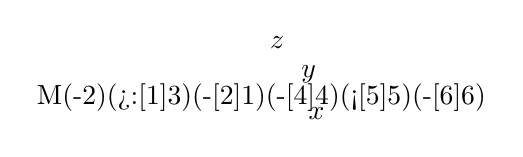
\begin{tikzpicture}
                \node {\chemfig{M(-2)(>:[1]3)(-[2]1)(-[4]4)(<[5]5)(-[6]6)}};
    
                \node at (0.7,-0.2) {$x$};
                \node at (0.6,0.3) {$y$};
                \node at (0.2,0.7) {$z$};
            \end{tikzpicture}
            \caption{Octahedral.}
            \label{fig:AOM-positionLabelinga}
        \end{subfigure}
        \begin{subfigure}[b]{0.3\linewidth}
            \centering
            \begin{tikzpicture}[
                every node/.style={black,fill=white,inner sep=1.5pt}
            ]
                \node {\chemfig{M(-)(>:[1])(-[2])(-[4])(<[5])(-[6])}};
    
                \draw [grx,semithick,dashed]
                    (-1.4,-1.4) rectangle (0.8,0.8)
                    (-0.8,-0.8) rectangle (1.4,1.4)
                    (-1.4,-1.4) -- (-0.8,-0.8) node{9}
                    (0.8,-1.4) node{10} -- (1.4,-0.8)
                    (0.8,0.8) -- (1.4,1.4) node{7}
                    (-1.4,0.8) node{8} -- (-0.8,1.4)
                ;
            \end{tikzpicture}
            \caption{Tetrahedral.}
            \label{fig:AOM-positionLabelingb}
        \end{subfigure}
        \begin{subfigure}[b]{0.3\linewidth}
            \centering
            \begin{tikzpicture}[
                every node/.style={black,fill=white,inner sep=1.5pt}
            ]
                \node {\chemfig{M(-2)(>:[1])(-[2]1)(-[4])(<[5])(-[6]6)}};
    
                \draw [grx,semithick,dashed]
                    (0.7,0) -- (-0.2,0.5) node[above left]{11} -- (-1.2,-0.5) node[below left]{12} -- cycle
                ;
            \end{tikzpicture}
            \caption{Trigonal bipyramidal.}
            \label{fig:AOM-positionLabelingc}
        \end{subfigure}
        \caption{Angular overlap model: Labeling of positions.}
        \label{fig:AOM-positionLabeling}
    \end{figure}
    \begin{itemize}
        \item With multiple ligands and multiple orbitals, we add the angular overlap interaction coefficients.
        \item These are tabulated for each orbital of each ligand at each position in the coordination sphere with each metal-center $d$-orbital.
        \item Suggested reading (on coefficients' derivation): \emph{TBD}.
    \end{itemize}
    \item Trigonal planar coordination example:
    \begin{itemize}
        \item From Figure \ref{fig:AOM-positionLabelingc}, the ligand positions are 2, 11, and 12.
        \item Thus, we add the coefficients in these rows to get $e_\sigma=(\frac{3}{4},\frac{9}{8},\frac{9}{8},0,0)$ and $e_\pi=(0,\frac{3}{2},\frac{3}{2},\frac{3}{2},\frac{3}{2})$, where the respective $d$-orbitals are $z^2,x^2-y^2,xy,xz,yz$.
        \item With these energies, we can now sum $e_\sigma+e_\pi$ to determine that the energies of the orbitals are $(\frac{3}{4},\frac{21}{8},\frac{21}{8},\frac{3}{2},\frac{3}{2})$.
        \item This gives us three sets of degenerate orbitals: Lowest energy ($d_{xz,yz}$), medium energy ($d_{z^2}$), and high energy ($d_{xy,x^2-y^2}$).
        \begin{itemize}
            \item How did we get these energy rankings?
        \end{itemize}
        \item Assigning Mulliken symbols with the $D_{3h}$ character table, we have from lowest to highest energy: $e''<a_1'<e'$.
    \end{itemize}
    \item Note that $e_\sigma$ is always positive (because ligands are $\sigma$-donors), but $e_\pi$ can be negative (because ligands can be $\pi$-acceptors).
    \item Changing the metal and/or ligand affects the magnitudes of $e_\sigma$ and $e_\pi$, thereby changing the value of $\Delta$.
    \item $e_\sigma>e_\pi$ always.
    \item Values decrease with increasing size and decreasing electronegativity.
    \item Both positive and negative values for $e_\pi$.
\end{itemize}



\section{Module 37: Jahn-Teller Effect}
\begin{itemize}
    \item The \textbf{Jahn-Teller theorem} helps explain why the $d^9$ configuration is far more stable (far higher peak) than predicted by Figure \ref{fig:CFSEcurve}.
    \item \textbf{Jahn-Teller theorem}: For nonlinear molecules/ions that have a degenerate ground-state, the molecule/ion will distort to remove the degeneracy. \emph{Also known as} \textbf{J-T theorem}.
    \begin{itemize}
        \item When orbitals in the same level are occupied by different numbers of electrons, this will lead to distortion of the molecule.
        \item If the two orbitals of the $e_g$ level have different numbers of electrons, this will lead to J-T distortion so as to stabilize the doubly occupied $e_g$ orbital and destabilize the singly occupied $e_g$ orbital.
        \item Cu(II) with its $d^9$ configuration is degenerate and has J-T distortion.
    \end{itemize}
    \item Consider the two degenrate $e_g$ orbitals ($d_{x^2-y^2,z^2}$).
    \emph{picture}
    \begin{itemize}
        \item Elongating the $z$-axis in an $O_h$ complex stabilizes the $d_{z^2}$ orbital and destabilizes the $d_{x^2-y^2}$ orbital.
        \item Vice versa for compressing the $z$-axis.
    \end{itemize}
    \item Thus, we can see significant elongation of the $z$-axis bonds in \ce{[Cu(H2O)6]^2+}.
    \item History: Before the rigorous formulation and verification of the J-T theorem by Jahn and Teller, Landau proposed the \textbf{Landau statement} from his observations.
    \item \textbf{Landau statement}: A molecule in an orbitally degenerate electronic state is unstable with respect to spontaneous distortion of the nuclear configuration that removes the degeneracy.
    \item Strength of the J-T effect in various configurations:
    \begin{table}[h!]
        \centering
        \renewcommand{\arraystretch}{1.4}
        \small
        \begin{tabular}{lcccccccccc}
            \noalign{\global\arrayrulewidth=1pt}\arrayrulecolor{grx}\hline
            Number of electrons & 1 & 2 & 3 & 4 & 5 & 6 & 7 & 8 & 9 & 10\\
            \rowcolor{grz}
            High-spin Jahn-Teller & w & w & & s & & w & w & & s & \\
            Low-spin Jahn-Teller & w & w & & w & w & & s & & s & \\
            \hline
        \end{tabular}
        \caption{Jahn-Teller effects in various configurations.}
        \label{tab:JTconfigurations}
    \end{table}
    \begin{itemize}
        \item Unequal occupation of $t_{2g}$ orbitals leads to the J-T effect in principle, but only weakly in practice because $t_{2g}$ orbitals are nonbonding in $\sigma$-bonded complexes, i.e., localized on the metal center, i.e., not strongly perturbed by ligand bonding.
        \item Unequal occupation of $e_g$ orbitals leads to a strong J-T effect since they are antibonding.
    \end{itemize}
    \item Structural effects of J-T distortion:
    \begin{itemize}
        \item In \ce{[Cu(en)2(H2O)2]^2+}, we will have axial aqua groups and equatorial en groups for two reasons.
        \begin{itemize}
            \item The aqua groups are weaker field ligands that interact less efficiently with the metal center, so it is easier for them to be farther from it.
            \item Having the en groups in plane means they don't have to be structurally distorted.
        \end{itemize}
        \item In \ce{[Cu(en)3]^2+}, we observe strong structural distortion from perfect octahedral forced by the J-T distortion; this angle strain is not energetically favorable.
    \end{itemize}
    \item Jahn-Teller distortion of the excited state:
    \begin{itemize}
        \item In high spin $d^6$ complexes such as \ce{[Fe(H2O)6]^2+}, there will only be weak J-T distortion of the ground state. Thus, we expect to see only one peak in the absorption spectrum, corresponding to the promotion of a $t_{2g}$ electron to the $e_g$ orbitals and its fall back down.
        \item However, we observe two bands.
        \item This is because promotion of an electron from the $t_{2g}$ orbitals to the $e_g$ orbitals leads to a much stronger J-T distortion (unequally occupied $e_g$ orbitals).
        \item The resultant $d$-orbital splitting causes the two absorption peaks.
    \end{itemize}
    \item Square planar complexes:
    \begin{itemize}
        \item Jahn-Teller distortion leads to tetragonal distortion of the octahedron, with the extreme of tetragonal distortion being the complete loss of axial ligands, and formation of a square-planar complex. Tetragonal distortion is the stretching of the axial \ce{M-L} bonds, and shortening of the in-plane bonds. \ce{Cu}(II) is usually tetragonally distorted, while low-spin \ce{Ni}(II) is usually square planar.
        \item Since the axial bonds get weaker as they lengthen, eventually we can have enough thermal energy to break them entirely, resulting in a square planar complex.
        \item This occurs in the case of \ce{Ni}(II) bonded to strong field ligands, such as cyano ligands. Essentially, what happens is the splitting of the $e_g$ orbitals exceeds the spin-pairing energy, causing the $d_{x^2-y^2}$ electron to pair with the $d_{z^2}$ electron.
        \begin{itemize}
            \item The filled $d_{z^2}$ orbital now occupies two coordination sites, and the four donor atoms occupy the plane.
            \item The structure is comparable to that of \ce{[IF4]-}, where two lone pairs occupy the axial sites.
            \item This is a particularly important special example because such compounds are very reactive, owing to their frontier $d_{z^2}$ orbitals, and can be involved in nucleophilic attacks.
        \end{itemize}
        \item All high-spin $d^8$ metal ions are octahedral (or tetrahedral). Low-spin $d^8$ metal ions are usually square planar.
        \item Both Wilkinson's catalyst and Crabtree's catalyst are square planar!
    \end{itemize}
\end{itemize}



\section{Module 38: Applying MO Theory Beyond "Simple" \ce{ML6} Complexes}
\begin{itemize}
    \item \marginnote{2/26:}Reviews Figure \ref{fig:orbitalDiagram-ML6} and the difference between $\pi$-acceptor and $\pi$-donor ligands.
    \item Mixing different ligands within the same coordination sphere:
    \begin{itemize}
        \item The MO diagram for $O_h$ complexes proves to be a convenient starting point for deducing the electronic structure of many lower symmetry metal complexes.
        \item To analyze lower symmetry compounds, we use the descent in symmetry technique.
    \end{itemize}
    \item \ce{[Co(CN)5Br]^3-} example:
    \begin{itemize}
        \item Five strong-field cyano ligands and one weak-field bromo ligand.
        \item Choose to orient the \ce{Br-} ligand along the positive $z$-axis.
        \item To build the MO, we could use DFT (first principles), but it's an unintuitive black box.
        \item Alternatively, we can start with hexacyanocobaltate(III), remove one cyano ligand and see how the MOs are perturbed, and add one bromo ligand and see how the MOs are perturbed. This process correlates the electronic structure of this $C_{4v}$ complex with its $O_h$ parent complex.
        \item To begin, consider perturbations to $\sigma$ and $\pi$ interactions upon substituting $\pi$-accepting \ce{CN-} with $\pi$-donating \ce{Br-}.
        \item First, let's simply remove the \ce{CN-} ligand.
        \begin{itemize}
            \item The $d_{x^2-y^2}$ orbital is not greatly perturbed by substitution along the $z$-axis.
            \item The $d_{z^2}$ orbital was \ce{M-L\sigma^*}; thus, removal of 1 $\sigma$ ligand from the $z$-axis will stabilize it.
            \item The $d_{xz,yz}$ orbitals are destabilized owing to the removal of 1 \ce{M-L\pi} bonding interaction.
            \item The $d_{xy}$ orbital is in-plane and nodal with respect to $\sigma$- and $\pi$-bonding along the $z$-axis; thus, it is not greatly perturbed by such substitution.
            \item The $d_{z^2}$ orbital is more greatly stabilized than the $d_{xz,yz}$ orbitals are destabilized because the former is involved in stronger $\sigma$-interactions, as opposed to weaker $\pi$-interactions.
        \end{itemize}
        \item Now let's add the \ce{Br-} ligand. Addition of \ce{Br-} to the $C_{4v}$ fragment will give rise to new interactions.
        \begin{itemize}
            \item $\sigma$: \ce{Br}($p_z$) will interact with the $d_{z^2}$, $s$, and $p_z$ orbitals of cobalt. All of these will be \ce{M-L\sigma^*} with respect to \ce{M} orbitals, and \ce{M-L\sigma} with respect to the ligand.
            \item $\pi$: \ce{Br}($p_x,p_y$) will interact with $d_{xz,yz}$ in \ce{M-L\pi^*} interactions.
            \item The formation of a bonding pair causes \ce{Br}($p_z$) orbital stabilization, at the cost of the destabilization of the $d_{z^2}$ orbital.
            \item The metal $p_z$ and $d_{z^2}$ orbitals will be destabilized, but will remain below \ce{Co-CN\sigma^*} orbitals because the \ce{Co-Br} interaction is not as great as the \ce{Co-CN} interaction.
        \end{itemize}
    \end{itemize}
\end{itemize}



\section{Module 39: Metal-Metal Bonding}
\begin{itemize}
    \item First historical puzzle:
    \begin{itemize}
        \item Copper (II) acetate has crystalizes with four \ce{O-CR-O} bridges joining two square pyramidal copper atoms that are also bonded to one aqua group, each.
        \item Copper is $d^9$, so $\mu=1.73$ in theory. However, we observe $\mu=1.4$.
        \item We resolve this conflict by noting that the copper atoms are not square pyramidal --- they bond to each other, giving both an octahedral geometry.
        \begin{itemize}
            \item This is important because it gives us a new pair of bonding and antibonding orbitals. We thus have low-spin and high-spin states, and the existence of a nonzero but not super high magnetic moment hints at a high-spin state with some preference for low-lyingness.
        \end{itemize}
    \end{itemize}
    \item Metal-metal bonding is common for metals in low oxidation state, and generally increases in strength along the series $3d<<4d<5d$.
    \item Single metal-metal bonded complexes:
    \begin{itemize}
        \item We will consider the paradiamagnetic single \ce{M-M} complex \ce{M2(CO)10}.
        \begin{itemize}
            \item Possible metals are \ce{Fe^2+}, manganese, and uranium.
        \end{itemize}
        \item Strategy for group fragment approach: Correlate to \ce{M(CO)6} ($O_h$), remove a ligand to give \ce{M(CO)5}, and dimerize.
        \begin{itemize}
            \item Note that \ce{Mn(CO)5} is the inorganic analog to \ce{CH3}, i.e., the \ce{Mn(CO)5} fragment is said to be isolobal with \ce{CH3}.
        \end{itemize}
        \item The HOMO of \ce{Mn(CO)5} is a singly occupied $d_{z^2}$ orbital.
        \item The energetic stabilization of the electrons in $d_{z^2}$ into a $\sigma$-bond by dimerization is the driving force for metal-metal bond formation.
        \item Note that a diamagnetic complex is formed from the dimerization of two metallic radicals.
        \item Also note that the $d_{z^2}$ orbital is cylindrically symmetric, i.e., indicates no preference for the staggered vs. eclipsed conformation. Thus, the molecule will adopt the more torsionally favorable staggered $D_{4d}$ configuration.
    \end{itemize}
    \item Cluster formation:
    \begin{itemize}
        \item As mentioned above, odd electron occupancy of the $e_g$ orbitals ($O_h$) prompts ligand loss in order to destabilize $d_{z^2}$. Further stabilization occurs by metal-metal single bond formation. We can take limiting argument to explain cluster formation across the periodic table:
        \item In each case, the clusters assume an octahedral coordination as a result of burying 7 $d$-electrons in what are formally $t_{2g}$ orbitals. The system loses a number of \ce{CO}s equivalent to the number of electrons in \ce{M-L\sigma^*}; this permits maximum \ce{M-M} bond formation and thus maximum stabilization.
        \item Clusters can trimerize or form higher polymers.
        \item Clusters can act as super atoms, combinations of atoms that you can add and remove electrons from with similar effects to changing the oxidation state in one atom.
    \end{itemize}
    \item Multiple metal-metal bonded complexes:
    \begin{itemize}
        \item Inorganic chemists synthesized a compound with a quadruple bond in 1964.
        \item The MO strategy will be to correlate \ce{Re2Cl8^2-} with \ce{ReCl6^3-} ($O_h$), remove two axial \ce{Cl-} ligands to give a square planar \ce{ReCl4-} fragment, and then dimerize.
        \begin{itemize}
            \item Here, we see stabilization of the $d_{xz,yz}$ (the \ce{Cl-} ligand had been giving antibonding character) orbitals and massive stabilization of the $d_{z^2}$ orbital (same reason).
        \end{itemize}
        \item The $d_{z^2}$ orbital reacts the most to form an $a_{1g}$ $\sigma$-bond.
        \item The $d_{xz,yz}$ orbitals react the second most to form two $e_u$ $\pi$-bonds.
        \item The $d_{xy}$ orbitals react the third most to form one $b_{2g}$ $\delta$-bond.
        \item The eclipsed $D_{4h}$ structure is a result of the $\delta$ bond.
        \item Adding up our 8 bonding and 0 antibonding electrons and diving by two gives us our first quadruple bond.
    \end{itemize}
    \item Metal-metal bonding vs. configuration: Increases single to quadruple bond as $d^1\to d^4$; decreases triple to no bond as $d^5\to d^8$.
    \item $f$ orbitals are deep within the core of the atom and not generally available form bonding, so we will not see higher bonding \emph{because} of $f$ orbitals in lanthanides and actinides.
    \item The $d^8$ case:
    \begin{itemize}
        \item No bonding predicted, but\dots
        \item We actually see one-dimensional crystals, as in band theory.
        \item The orbitals responsible are the $d_{z^2}$ orbitals, which mix with the higher energy $p_z$ orbitals to stabilize the $d_{z^2}$ $\sigma$-bonding MO (and destabilize the $p_z$ bonding MO, but this orbital is unfilled).
    \end{itemize}
    \item The $d_{x^2-y^2}$ orbitals cannot participate in \ce{ML4} coupling since they are used for ligand bonding.
    \begin{itemize}
        \item Thus, the only orbitals available for coupling are $d_{z^2,xz,yz,xy}$.
    \end{itemize}
    \item Inorganic chemists (including Phil Power, who is probably the greatest currently living main-group inorganic chemist) synthesized a compound with a quintuple bond in 2005.
    \begin{itemize}
        \item They had to change the coordination environment around the metal center to free up the $d_{x^2-y^2}$ orbital. They did so with sterically bulky ligands that hindered more bonding.
        \item The quintuple bonding was verified by observing a very short bond length (not super short on the scheme of things, but shorter than ever reported before, indicating the presence of a weak fifth bond).
        \item $C_{2h}$ symmetry.
        \item Suggested reading: The full paper.
    \end{itemize}
\end{itemize}



\section{Chapter 10: Coordination Chemistry II (Bonding)}
\emph{From \textcite{bib:MiesslerFischerTarr}.}
\begin{itemize}
    \item \marginnote{3/3:}We seek to review experimental observations of coordination complexes and show how these observations have been reconciled with electronic structure and bonding theories.
    \item \textbf{Stability constant}: An equilibrium constant in a reaction that forms a coordination complex, typically by replacing one or more aqua ligands with another type. \emph{Also known as} \textbf{formation constant}.
    \begin{itemize}
        \item A measure of bond strength frequently used by inorganic chemists.
    \end{itemize}
    \item Stronger field ligands preferably bond to the metal center.
    \item Polydentate ligands bond more readily than one split into chunks each with fewer attachment sites because bonding once makes bonding a second time easier (proximity), and ligand dissociation is more difficult.
    \begin{itemize}
        \item Thus, for example, \ce{[Ni(en)3]^2+} is more stable than \ce{[Ni(CH3NH2)6]^2+}.
    \end{itemize}
    \item The chelate effect has the largest impact on formation constants when the ring is 5-6 atoms long (shorter causes strain; longer means less proximity, hence tougher bond formation).
    \item "Thermodynamic parameters such as $\Delta H^\circ$, $\Delta S^\circ$, and the dependence of $K$ with $T$ are useful for comparing reactions of different metal ions reacting with the same ligand or a series of different ligands reacting with the same metal ion" \parencite[358]{bib:MiesslerFischerTarr}.
    \begin{itemize}
        \item Sometimes, properties of coordination complexes can be predicted directly off of this information, but it's rare.
    \end{itemize}
    \item An example of the thermodynamics of the chelate effect:
    \begin{gather*}
        \ce{[Cd(H2O)6]^2+ + 4CH3NH2 -> [Cd(CH3NH2)4(H2O)2]^2+ + 4H2O}\tag*{$K=\num{3.3e6}$}\\
        \ce{[Cd(H2O)6]^2+ + 2en -> [Cd(en)2(H2O)2]^2+ + 4H2O}\tag*{$K=\num{4.0e10}$}
    \end{gather*}
    \begin{itemize}
        \item Differences in $\Delta S^\circ$ play the dominant role in the chelate effect. $\Delta H^\circ$ is similar for the above two reactions, but for the en substitution, we dramatically increase entropy by binding two en particles and liberate four \ce{H2O} particles, as opposed to conserving the number of particles in the methylamine reaction.
    \end{itemize}
    \item \textbf{Magnetic susceptibility}: A molecule's attraction to or repulsion from a magnetic field. \emph{Also known as} $\bm{\chi}$.
    \item $\mu=2.828\sqrt{\chi T}$, where $2.828\approx\sqrt{3k/N}$.
    \item "The total spin magnetic moment for a configuration of electrons is characterized by the spin quantum number $S$, which is equal to the maximum total spin, the sum of the $m_s$ values" \parencite[360]{bib:MiesslerFischerTarr}.
    \item "The orbital angular momentum [is] characterized by the quantum number $L$, where $L$ is equal to the maximum possible sum of the $m_l$ values for an electronic configuration" \parencite[360]{bib:MiesslerFischerTarr}.
    \begin{itemize}
        \item For a $p^4$ ground state electron configuration, $L$ is maximized when two electrons occupy the orbital with $m_l=+1$, and the other two occupy the $m_l=0,-1$ orbitals, respectively. Thus, $L_{p^4}=1+1+0-1=1$.
    \end{itemize}
    \item Technically, $\mu_S=2.00023\sqrt{S(S+1)}$ where $2.00023$ is the gyromagnetic ratio.
    \begin{itemize}
        \item However, if we round the gyromagnetic ratio to 2 and note that $S=\frac{n}{2}$ where $n$ is the number of unpaired electrons, we obtain $\mu_S=\sqrt{n(n+2)}$.
    \end{itemize}
    \item Recall from Chapter 2 that in transition metals, $ns$ electrons are lost before $(n-1)d$ electrons.
    \item Number of unpaired electrons examples:
    \begin{itemize}
        \item \ce{Fe} is $4s^23d^6$, so 4 unpaired $d$-electrons.
        \item \ce{Fe^2+} is $3d^6$, so 4 unpaired $d$-electrons.
        \item \ce{Cr} is $4s^13d^5$, so 6 unpaired electrons (1 unpaired $s$-electron and 5 unpaired $d$-electrons).
        \item \ce{Cu} is $4s^13d^{10}$, so 1 unpaired $s$-electron.
        \item \ce{Cu} is $3d^9$, so 1 unpaired $d$-electron.
    \end{itemize}
    \item The unit symbol for Bohr magnetons is $\mu_B$, so we say, for instance, that the magnetic moment of copper is $\SI{1.73}{\mu_B}$.
    \item \textcite{bib:MiesslerFischerTarr} gives a full explanation of the Gouy method.
    \begin{itemize}
        \item Modern magnetic susceptibility measurements are taken with a magnetic susceptibility balance (for solids), via the Evans NMR method (for solutes), or with a SQUID.
    \end{itemize}
    \item \textbf{Mass susceptibility}: The magnetic susceptibility of a substance per gram.
    \item "A complex with one unpaired electron exhibits ideal \textbf{Curie paramagnetism} if the inverse of the molar susceptibility (for a given applied external field) increases linearly with temperature and has a $y$-intercept of 0" \parencite[362]{bib:MiesslerFischerTarr}.
    \item "In a paramagnetic complex, the magnetic moments of individual species do not effectively couple, but act more or less independently of each other" \parencite[362]{bib:MiesslerFischerTarr}.
    \begin{itemize}
        \item This contrasts with ferromagnetism.
    \end{itemize}
    \item \textbf{Antiferromagnetism}: An alternate long-range arrangement of magnetic moments where adjacent moments line up in opposite directions.
    \item Electronic spectra and molecular shapes provide further evidence for electronic structures.
    \item There are three main bonding models for coordination complexes.
    \item \textbf{Crystal field theory}: This is an electrostatic approach, used to describe the split in metal $d$-orbital energies within an octahedral environment. It provides an approximate description of the electronic energy levels often responsible for the ultraviolet and visible spectra of coordination complexes, but it does not describe metal-ligand bonding.
    \item \textbf{Ligand field theory}: This is a description of bonding in terms of the interactions between metal and ligand frontier orbitals to form molecular orbitals. It uses some crystal field theory terminology but focuses on orbital interactions rather than attractions between ions.
    \item \textbf{Angular overlap method}: This is a method of estimating the relative magnitudes of molecular orbital energies within coordination complexes. It explicitly takes into account the orbitals responsible for ligand binding as well as the relative orientation of the frontier orbitals.
    \item \textbf{Born-Oppenheimer approximation}: Atomic nuclei are in fixed positions in comparison with rapidly moving electrons.
    \item \textbf{Extended H\"{u}ckel theory}: The simplest approach to approximating the many-body problem of electronic movements.
    \pagebreak
    \item Thoughts on CFT:
    \begin{itemize}
        \item "When the $d$ orbitals of a metal ion are placed in an occtahedral field of ligand electron pairs, any electrons in these orbitals are repelled by the field. As a result, the $d_{x^2-y^2}$ and $d_{z^2}$ orbitals, which have $e_g$ symmetry, are directed at the surrounding ligands and are raised in energy. The $d_{xy}$, $d_{xz}$, and $d_{yz}$, orbitals ($t_{2g}$ symmetry), directed between the ligands, are relatively unaffected by the field" \parencite[364]{bib:MiesslerFischerTarr}.
        \item In $\Delta_o$, the $o$ stands for octahedral.
        \begin{figure}[h!]
            \centering
            \begin{tikzpicture}[
                yscale=0.8,
                semithick,
                every node/.append style={black}
            ]
                \footnotesize
                \draw [dash pattern=on 5mm off 2mm]
                    (0,0) -- node[below=2mm]{Free ion} ++(3.3,0)
                    (4,2) -- node[below=1.8cm]{Spherical field} ++(3.3,0)
                    (8,0) -- node[below=2mm]{Octahedral field} ++(1.9,0) node[right]{$t_{2g}$}
                    (8.35,5) -- ++(1.2,0) node[right]{$e_g$}
                ;
                \draw [grx,densely dashed]
                    (3.3,0) -- (4,2)
                    (3.3,0) -- (8,0)
                    (7.3,2) -- (8,0)
                    (7.3,2) -- (9.55,2)
                    (7.3,2) -- (8.35,5)
                ;
        
                \draw [grx,stealth-stealth] (8.95,0.05) -- node[right]{$0.4\Delta_o$} ++(0,1.9);
                \draw [grx,stealth-stealth] (8.95,2.05) -- node[right]{$0.6\Delta_o$} ++(0,2.9);
                \draw [grx,stealth-stealth] (10.8,0.05) -- node[right]{$\Delta_o$} ++(0,4.9);
            \end{tikzpicture}
            \caption{Crystal field splitting from the free ion.}
            \label{fig:CFT-freeIon}
        \end{figure}
        \item "The average energy of the five $d$ orbitals [in a coordination complex] is above that of the free ion orbitals [i.e., those in the metal ion before it is surrounded by ligands], because the electrostatic field of the ligands raises their energy" \parencite[364]{bib:MiesslerFischerTarr}.
        \item CFT is flawed because as we can see from Figure \ref{fig:CFT-freeIon}, there is no energetically favorable bonding; at best, we could have zero energy difference between the free ion and bonded octahedral field state (this occurs if only the $t_{2g}$ orbitals are occupied).
    \end{itemize}
    \item \marginnote{3/4:}Ligand field theory was synthesized from CFT and MO theory by Griffith and Orgel.
    \item The ligand HOMO often serves as the basis for group orbitals.
    \item Based on their shapes, it makes sense that the symmetry of the $d_{xy,xz,yz}$ orbitals doesn't match that of the ligand $\sigma$ orbitals.
    \item The colors of transition metal complexes are often due to the energy difference between the $t_{2g}$ and ${e_g}^*$ orbitals, which is often equal to the energy of photons of visible light.
    \begin{itemize}
        \item \ce{[Ni(H2O)6]^2+}, for example, is green because $\Delta_o$ matches well with the energy of red light, so when white light passes through a solution of this compound, red light is absorbed and the complement (green light) passes through to be perceived.
    \end{itemize}
    \item "$\Delta_o$ is also used in ligand field theory as a measure of the magnitude of metal-ligand interactions" \parencite[367]{bib:MiesslerFischerTarr}.
    \item Perhaps the orbital labeling scheme in Figure \ref{fig:piOctahedralLigand} isn't actually procedural; it's just a consistent reference frame.
    \item The interaction of ligand $\pi$($t_{1u}$) orbitals with metal $p$($T_{1u}$) orbitals is relatively weak since metal $p$ orbitals largely interact with ligand $\sigma$($t_{1u}$) orbitals.
    \item "Strong $\pi$ acceptor ligands have the ability to increase the magnitude of $\Delta_o$ by lowering the energy of the $t_{2g}$ orbitals" \parencite[368]{bib:MiesslerFischerTarr}.
    \item "Electrons in the lower bonding orbitals are largely concentrated on the ligands. It is the stabilization of these ligand electrons that is primarily responsible for why these ligands bind to the metal center" \parencite[368]{bib:MiesslerFischerTarr}.
    \item Electrons in higher energy orbitals are affected by ligand field effects and determine "structural details, magnetic properties, electronic spectrum absorptions, and coordination complex reactivity" \parencite[368]{bib:MiesslerFischerTarr}.
    \item \textbf{Metal-to-ligand (\ce{M -> L}) $\bm{\pi}$ bonding}: Electron donation from metal $d_{xy,xz,yz}$ orbitals to ligand $\pi^*$ orbitals. \emph{Also known as} \textbf{$\bm{\pi}$ back-bonding}.
    \item $\Delta_o$ is the splitting between the \emph{highest occupied} $t_{2g}$ (which can be either $t_{2g}$ or ${t_{2g}}^*$) orbital and the ${e_g}^*$ orbital.
    \begin{figure}[h!]
        \centering
        \begin{tikzpicture}[
            yscale=0.8,
            semithick
        ]
            \footnotesize
            \draw [dash pattern=on 4mm off 1mm]
                (0,2) -- node[below]{$t_{2g}$} node[below=4mm,text width=9mm]{Empty ligand group orbital} ++(1.4,0) coordinate (pl)
                (5,-3.5) coordinate (sl) -- node[below]{$t_{2g}$} node[below=4mm,text width=1.1cm]{$\sigma$ bonds only} node[pos=0.143,above]{$\uparrow$} node[pos=0.5,above]{$\uparrow$} node[pos=0.857,above]{$\uparrow$} ++(1.4,0) coordinate (sr)
                (10,-4) coordinate (pr) -- node[below]{$t_{2g}$} node[below=4mm,text width=9mm]{Filled ligand group orbital} node[pos=0.143,above]{$\uparrow$$\downarrow$} node[pos=0.5,above]{$\uparrow$$\downarrow$} node[pos=0.857,above]{$\uparrow$$\downarrow$} ++(1.4,0)
                (2,3.5) coordinate (t2glul) -- node[below]{${t_{2g}}^*$} ++(1.4,0) coordinate (t2glur)
                (2,-5) coordinate (t2glll) -- node[below]{$t_{2g}$} node[pos=0.143,above]{$\uparrow$} node[pos=0.5,above]{$\uparrow$} node[pos=0.857,above]{$\uparrow$} ++(1.4,0) coordinate (t2gllr)
                (8,-2) coordinate (t2grul) -- node[below]{${t_{2g}}^*$} node[pos=0.143,above]{$\uparrow$} node[pos=0.5,above]{$\uparrow$} node[pos=0.857,above]{$\uparrow$} ++(1.4,0) coordinate (t2grur)
                (8,-6.5) coordinate (t2grll) -- node[below]{$t_{2g}$} node[pos=0.143,above]{$\uparrow$$\downarrow$} node[pos=0.5,above]{$\uparrow$$\downarrow$} node[pos=0.857,above]{$\uparrow$$\downarrow$}  ++(1.4,0) coordinate (t2grlr)
                (2.25,0) -- node[below]{${e_g}^*$} ++(0.9,0) coordinate (egl)
                (5.25,0) coordinate (egml) -- node[below]{${e_g}^*$} ++(0.9,0) coordinate (egmr)
                (8.25,0) coordinate (egr) -- node[below]{${e_g}^*$} ++(0.9,0)
            ;
            \draw [grx,densely dashed]
                (pl) -- (t2glul)
                (pl) -- (t2glll)
                (t2glur) -- (sl)
                (t2gllr) -- (sl)
                (sr) -- (t2grul)
                (sr) -- (t2grll)
                (t2grur) -- (pr)
                (t2grlr) -- (pr)
                (egl) -- (egml)
                (egmr) -- (egr)
            ;
    
            \draw [-stealth] (t2gllr) -- node[right]{$\Delta_o$} (t2gllr |- egl);
            \draw [-stealth] (sr) -- node[right]{$\Delta_o$} (sr |- egmr);
            \draw [-stealth] (t2grur) -- node[right]{$\Delta_o$} (t2grur |- egr);
        \end{tikzpicture}
        \caption{Effects of $\pi$ bonding on $\Delta_o$ using a $d^3$ ion.}
        \label{fig:piDeltao}
    \end{figure}
    \begin{itemize}
        \item This is why we consider $\Delta_o$ to be the energy difference between the $t_{2g}$ and ${e_g}^*$ orbitals in complexes with $\pi$-accepting ligands (where the $t_{2g}$ orbitals are filled and lie beneath the ${e_g}^*$ orbitals), but the difference between the ${t_{2g}}^*$ and ${e_g}^*$ orbitals in complexes with $\pi$-donating ligands (where the $t_{2g}$ \emph{and} ${t_{2g}}^*$ are filled and \emph{both} lie beneath the ${e_g}^*$ orbitals).
        \item Empty ligand group orbitals engage in \ce{M -> L} bonding while filled ligand group orbitals engage in \textbf{\ce{L -> M} bonding}.
    \end{itemize}
    \item \textbf{Ligand-to-metal (\ce{L -> M}) $\bm{\pi}$ bonding}: Electron donation from the ligand $\pi$ orbitals to metal $d_{xy,xz,yz}$ orbitals.
    \item \ce{L -> M} bonding favors high-spin configurations while \ce{M -> L} bonding favors low-spin configurations.
    \item Part of the stabilization of \ce{M -> L} bonding comes from donation of excess electron density on the metal cation resulting from $\sigma$ acceptance back to the ligands (metals prefer to be relatively positive because of their low electronegativity).
    \item Note that because backbonding orbitals are composed of $\pi^*$ orbitals, filling of them results in weakening of the ligand $\pi$ bond.
    \item "In octahedral coordination complexes, electrons from the ligands fill all six bonding molecular orbitals, and the metal valence electrons occupy the $t_{2g}$ and $e_g^*$ orbitals" \parencite[372]{bib:MiesslerFischerTarr}.
    \item Strong field ligands interact more strongly with metal orbitals, leading to greater stabilization of the $t_{2g}$ set, leading to a larger $\Delta_o$ and low-spin configurations.
    \begin{itemize}
        \item Weak field ligands interact more weakly metal orbitals, leading to lesser stabilization of the $t_{2g}$ set, leading to a smaller $\Delta_o$ and low-spin configurations.
    \end{itemize}
    \item Recall that increases in $\Pi_c$ \emph{destabilize} the complex, whereas increases in $\Pi_e$ \emph{stabilize} the complex.
    \item Is there any case in which we would have a $d^5$ configuration with four $t_{2g}$ electrons and one ${e_g}^*$ electron?
    \item \ce{Co^3+} is the third row cation that most easily adopts a low-spin configuration.
    \item Magnitudes of $\Delta_o$ values:
    \begin{itemize}
        \item Values for $d^5$ ions are smaller than those of $d^4$ and $d^6$ ions.
        \item Increases in the principal quantum number $n$ increase $\Delta_o$ because of two effects:
        \begin{itemize}
            \item There is greater overlap between the larger $4d$ and $5d$ orbitals and the ligand orbitals.
            \item There is a decreased pairing energy due to a larger available volume for electrons in the $4d$ and $5d$ orbitals relative to with $3d$ orbitals.
        \end{itemize}
    \end{itemize}
    \item \textbf{Ligand field stabilization energy}: The difference\footnote{This is equivalent to the CFSE defined in the lecture.} between the energy of the $t_{2g}$ / $e_g$ electronic configuration resulting from the ligand field splitting and the hypothetical energy of the $t_{2g}$ / $e_g$ electronic configuration with all five orbitals degenerate and equally populated. \emph{Also known as} \textbf{LFSE}.
    \item Note that LFSE can only be calculated using the $\frac{2}{5}$ / $\frac{3}{5}$ method for $\sigma$-bonded octahedral complexes.
    \item Although we might expect transition metal ions to have linearly\footnote{Errata: \textcite{bib:MiesslerFischerTarr} refers to the linear line in the graph as "blue," even though it should be green (a relic from the previous edition).} increasingly exothermic $\Delta H$s for hydration reactions (see below) across a period (as decreasing atomic radius makes them more concentrated [hence more unstable] sources of postive charge), we observe two loops similar to Figure \ref{fig:CFSEcurve} but inverted.
    \begin{equation*}
        \ce{M^2+ + 6H2O -> [M(H2O)6]^2+}
    \end{equation*}
    \begin{itemize}
        \item This is because the LFSE provides extra stabilization.
        \item It is also because of spin-orbit coupling, a relaxation effect caused by contraction of the metal-ligand distance, and an interelectronic repulsion energy (see Chapter 11 for a more detailed description of the first and third phenomena).
        \item Small corrections must be made in cases where the J-T distortion is present.
    \end{itemize}
    \item \textbf{Nephelauxetic effect}: The magnitude of the reduction in the interelectron repulsion energy between the free ion and coordination complex.
    \begin{itemize}
        \item Is this due to increases in delocalization?
        \item Factors that increase the nephelauxetic effect:
        \begin{itemize}
            \item Softness of the ligand.
            \item Increase in metal oxidation state magnitude.
        \end{itemize}
    \end{itemize}
\end{itemize}




\end{document}